\documentclass[11pt,a4paper]{article}
\usepackage[utf8]{inputenc}
\usepackage{amsmath}
\usepackage{amsfonts}
\usepackage{amssymb}
\usepackage{graphicx}
\usepackage{float}
\usepackage{url}
\usepackage{amsmath}
\usepackage{amsthm}
\usepackage{amssymb}
\usepackage[francais]{babel}

\usepackage[left=3cm,right=3cm,top=3cm,bottom=3cm]{geometry}

\newtheorem{thm}{Theorem}
\newtheorem{prop}{Propriété}

\theoremstyle{definition}
\newtheorem{defn}{Définition}

\theoremstyle{remark}
\newtheorem{rmq}{Remarque}

\theoremstyle{remark}
\newtheorem{ex}{Exemple}


\author{Pimprenelle Parmentier}



\title{Stream graphes multicouches}
\begin{document}
\begin{titlepage}


\noindent
\textsc{Ecole polytechnique}\\
PROMOTION X2016 \\
MASTER: Mathématiques appliquées\\
PARMENTIER Pimprenelle

\vspace{3cm}
\begin{center}
\textsc{\Large Rapport de stage}
\vspace{1cm}
\hrule % Horizontal line
\vspace{0.4cm}
{\huge \bfseries Stream graphes multicouches \par}\vspace{0.4cm} % Thesis title
\hrule 
\vspace{1cm}
\textsc{\Large Rapport non confidentiel}
\vspace{4cm} % Horizontal line
 
\end{center}

\noindent
\textit{Option:} Département de Mathématiques appliquées\\
\textit{Champ:} Etude de graphes\\
\textit{Enseignant référent:} Xavier ALLAMIGEON\\
\textit{Tuteur de stage dans l'organisme:} Tiphaine VIARD\\
\textit {Co-tuteurs de stage hors organisme:} Benjamin RENOUST (Université d'Osaka)\\
\hspace*{6.1cm} Jean-François Baffier (JSPS)\\
\textit{Dates du stage:} 8 avril 2019 - 23 aout 2019\\
\textit{Adresse de l'organisme:}\\
RIKEN AIP\\
Nihonbashi 1-chome Mitsui,\\
Building, 15th floor,\\
1-4-1 Nihonbashi,\\
Chuo-ku, Tokyo\\
103-0027, Japan\\
\end{titlepage}


\begin{abstract}

\end{abstract}



\newpage 

\tableofcontents
\newpage



\section*{Introduction}

\section{Etat de l'art}
\indent

Les graphes s'écrivent sous la forme $G=(V,E)$ et servent à modéliser des interactions (arêtes : ensemble $E$) entre des entités (nœuds: ensemble $V$). 

\begin{figure}[H]
	\centering
	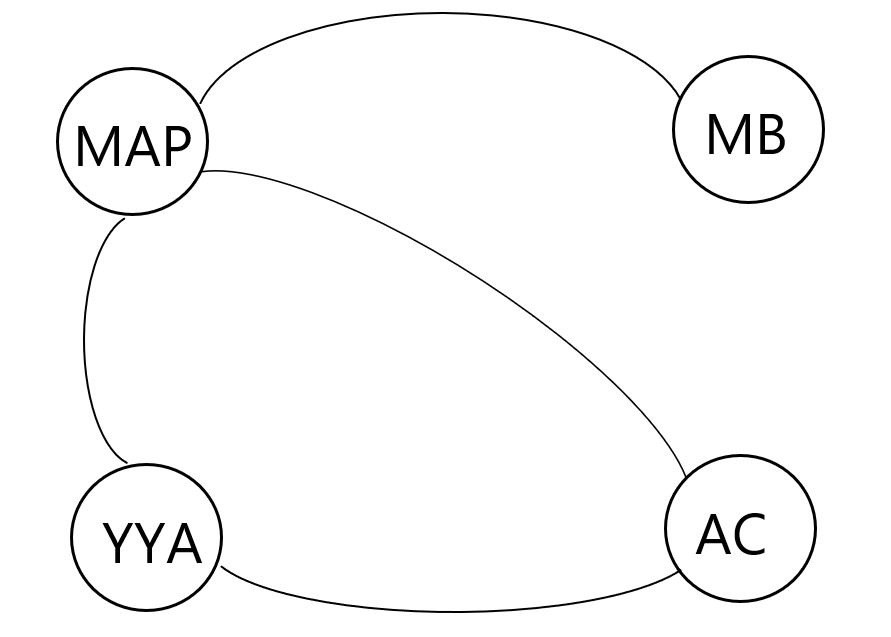
\includegraphics[width=0.3\textwidth]{exGraphe.JPG}
	\caption{Un exemple de graphe de connaissance. Les chercheurs MAP, AC et YYA se connaissent, les chercheurs MB et MAP aussi. En revanche, il n'y a pas de lien entre MB et AC, qui ne se connaissent donc pas.}
\end{figure}

\subsection{Les graphes multicouches}

\subsubsection{Définition générale}

 Les graphes multicouches sont utilisés pour décrire des interactions entre des noeuds qui peuvent être de différentes natures de façon simultanée et/ou qui peuvent avoir des interactions de natures différentes. 
 
 Une définition très générale des graphes multicouches est donnée dans le papier \cite{mlkiv}, nous la résumons ici.
 
 La structure d'un graphe multicouches est décrite par le k-uplet d'ensembles ${\cal L} = L_1, \dots , L_k$. Chaque $L_i$ est un ensemble d'attributs que peut avoir une couche, appelés "couches élémentaires". Chaque couche correspond donc à un élément de $L=L_1\times L_2 \times \dots \times L_k$.
 
 Un graphe multicouches s'écrit alors $M = (V_M, E_M, V, L)$. $V$ est l'ensemble de ses noeuds, $L$ la structure des couches, $V_M$ sont les noeuds-couches, qui comme leur nom l'indique, sont les éléments de $V\times L$. Enfin $E_M \subseteq V_M \times V_M $ est l'ensemble des liens, un lien pouvant relier deux noeuds-couches entre eux. 

\begin{figure}[H]
	\centering
	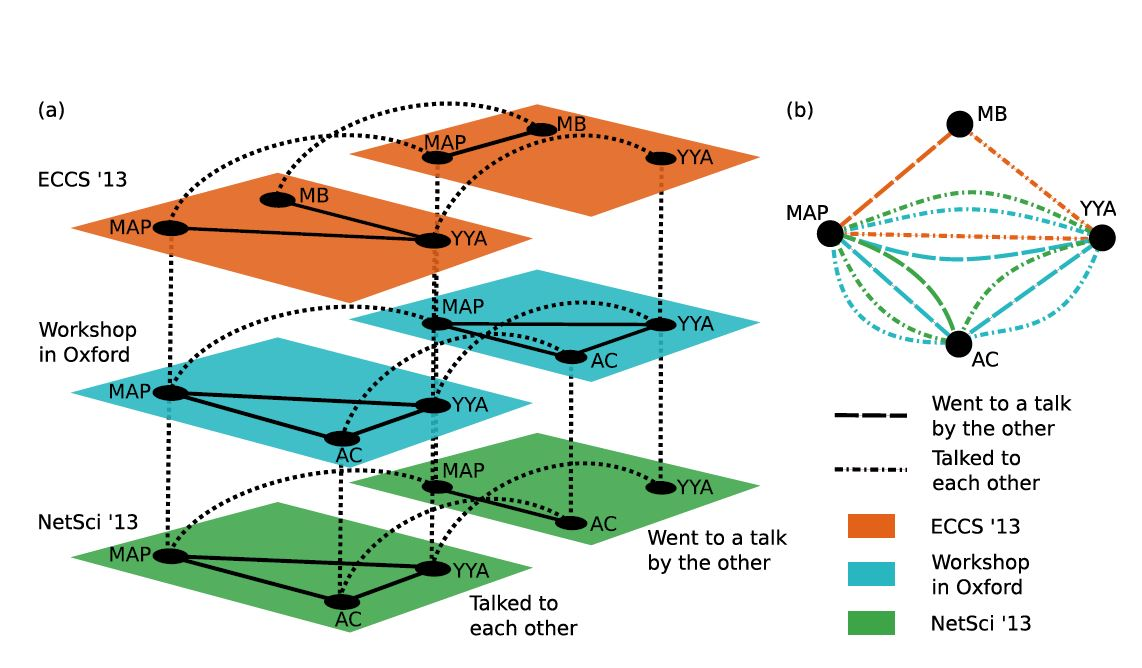
\includegraphics[width=0.6\textwidth]{exmultilayer.JPG}
	\caption{\textbf{Un exemple de graphe multicouches} extrait de \cite{mlkiv}. Ici, les noeuds sont des chercheurs représentés par leurs initiales: $V = \{MAP,MB,YYA,AC\}$. Chaque couche est caractérisée par une conférence et un type de relation: $L = \{$conferences, relationship types$\}$. Les noeuds couches existent ou non en fonction de la présence ou non d'un chercheur à une conférence: $V_M$ contient par exemple (MAP;ECCS'13,Talked to each other). Enfin, les liens représentent les interaction entre les chercheurs à des conférences précises: $E_M$ contient par exemple ((MAP;ECCS'13,Taked to each other),(YYA;ECCS'13,Talk to each other)). }

\end{figure}

\subsubsection{Cadres d'utilisation}


Les graphes multicouches trouvent de nombreuses applications, par exemple en \textbf{écologie} \cite{ecolo} (les noeuds sont alors des espèces ou des individus, les couches élémentaires des types d'interaction (parasite, prédateur...), des lieux, des temps, etc. On cherche alors à savoir comment se diffuse une maladie, quelles sont les faiblesses d'un écosystèmes (quels sont les liens / nœuds qui assurent le bon fonctionnement ?)

Un autre jeu de données utilisé est en \textbf{économie}, celui des interactions entre les banques européennes, les couches étant caractérisées par le type d'interaction (de "prêt"), les noeuds étant les banques et un lien existant entre deux banques de la même couche quand celles-ci procèdent à une interaction du type correspondant.

Un dernier exemple intuitif est celui des \textbf{réseaux de transport}, dans lequel les couches sont les différents moyens de transport possible, les nœuds sont des localités et les liens les différentes lignes de transport. Un tel jeu de données peut être trouvé sur le site gouvernemental américain des statistiques de transport, pour les lignes aériennes \cite{plane}.

On remarque que dans beaucoup de situations, nous avons des liens "implicites" entre tous les différents noeuds-couches issus du même noeud, et des liens "explicites" ne pouvant apparaitre qu'au sein d'une même couche. De tels graphes sont appelés \textbf{multiplexes}.





%Ils permettent de représenter des graphes de collaboration entre chercheurs par exemple : chaque chercheur collabore avec d'autres sur des mots-cles précis, les noeuds sont alors les chercheurs, les couches les différents mots-clés utilisés et des liens apparaissent entre deux chercheurs-mots clés quand les deux chercheurs apparaissent sur le même papier traitant du mot-clé.

\subsubsection{Quelques définitions}

\begin{defn}{\textbf{Tenseur d'adjacence}}
	
\end{defn}
D'un point de vue pratique, ces graphes peuvent être manipulés à l'aide de tenseurs d'adjacence \cite{mldd}, d'ordre 4. Chaque élément $M^{u,\alpha}_{v,\beta}$ indique s'il existe un lien entre les nœuds-couches $(u,\alpha)$ et $(v,\beta)$.

\begin{defn}{\textbf{Arêtes intra-couches et inter-couches.}}
	On appelle arêtes inter-couches les arêtes qui lient deux nœud-couches de couches différentes. (L'ensemble des arêtes inter-couches s'écrit $E_A = \{((u,\alpha),(v,\beta)) \in E_M | \alpha = \beta\}$). On appelle arêtes intra-couches les arêtes qui lient deux noeuds-couches de la même couche. (L'ensemble correspondant s'écrit $E_C = E_M\backslash E_A$).
\end{defn}
Ainsi, les multiplexes sont des graphes multicouches dans lesquels les seuls arêtes intercouches autorisées sont les arêtes entre les noeuds-couches du même noeud.

\begin{defn}{\textbf{Graphe agrégé}}
	On appelle le graphe aggrégé le graphe qu'on obtient en "superposant" les couches d'un graphe multicouches : $$G=(V_G,E_G), \quad V_G=V, \quad E_G={(u,v)|\exists \alpha, \beta | ((u,\alpha),(v,\beta)) \in E_M}$$.
\end{defn}

\begin{defn}{\textbf{Graphe sous-jacent}}
Le graphe sous-jacent de $M$ est le graphe qu'on obtient en faisant abstraction de la structure multicouches, et dans lequel chaque noeud est un noeud-couche.
$$G=(V_{SJ},E_{SJ}), \quad V_{SJ} = V_M, \quad E_{SJ}=E_M$$
\end{defn}




\subsubsection{Pourquoi utiliser des graphes multicouches à la place de graphes ?}

On remarque que dans beaucoup de cas, les graphes sont des graphes agrégés ou sous-jacent de graphes multicouches. Une partie de l'information a été "perdue" mais cela permet d'utiliser des outils très puissants et d'obtenir des résultats déjà satisfaisants grâce à la théorie des graphes. On peut donc se demander quel est l'intérêt d'utiliser ce formalisme, et de garder une telle quantité d'informations. De nouvelles mesures et de nouveaux algorithmes ont donc été créés pour pouvoir analyser plus finement ces informations plus détaillées.

En voici deux exemple, qui seront source d'inspiration dans la suite sur ce qu'il sera possible de faire avec l'objet que nous allons introduire.


\paragraph{Importance de la structure : Isomorphismes de graphes}

Deux graphes $G_1$ et $G_2$ sont dits isomorphes quand on peut trouver une bijection des sommets du premier graphes vers ceux du second qui préserve les arêtes.


\begin{figure}
\centering
	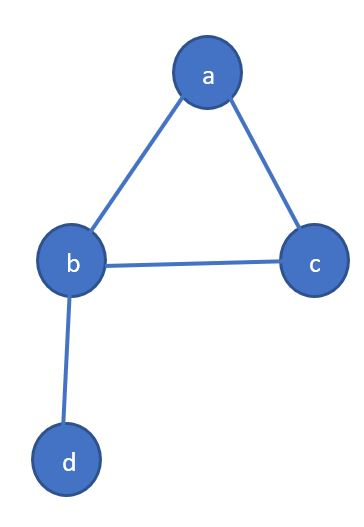
\includegraphics[width=0.2\textwidth]{graph1iso.JPG}
	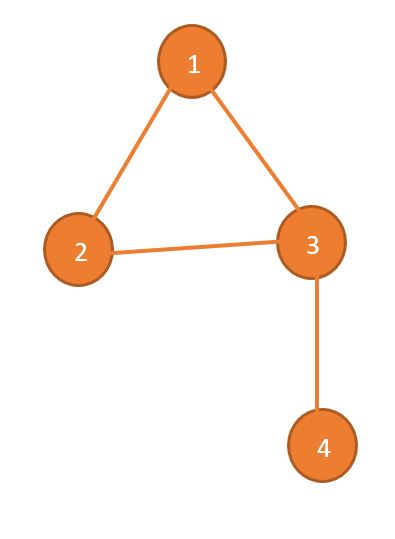
\includegraphics[width=0.2\textwidth]{graph2iso.JPG} 
	
	\caption{Un exemple de deux graphes isomorphes : $\sigma(a)=1, \sigma(b)=3, \sigma(c)=2, \sigma(d)=4$}
\end{figure}

Dans le cadre des multicouches, Kivelä et Porter \cite{isoMulti} définissent l'automorphisme de graphe (sans perte de généralité) par une permutation des arêtes, des couches élémentaires et des couches qui préserve les liens.


Kiveä et Porter démontrent qu'il n'est pas équivalent de dire que deux graphes multicouches sont isomorphes et leurs graphes sous-jacent sont équivalents. En effet, il ne faut pas perdre de vue que la structure "arborescente" des couches, doit être conservée, et pas seulement l'idée de "partition" des nœuds en différentes couches. Ils présentent un algorithme permettant de vérifier si deux graphes multicouches sont isomorphes.

\paragraph{Centralité}

La question de la centralité a été traitée dans \cite{centraliteMulti}. De Domenico met en avant le fait qu'il est "réducteur" de calculer des centralités sur des graphes agrégés pour trouver quels sont les noeuds ayant les roles les plus centraux dans la cohésion de l'ensemble d'une structure. Ils définissent donc un nouveau "PageRank" et une nouvelle centralité intermédiaire (betweeness centrality). Le PageRank est calculé à partir du tenseur d'adjacence du graphe, on obtient alors des centralités pour chaque noeud-couche, qu'on traite de la manière la plus adaptée en fonction du problème à résoudre.

La centralité intermédiaire est calculée en sommant les centralités intermédiaires des différents nœuds-couches.

De Domenico montre que le fait de conserver l'information multicouche permet de trouver un classement des noeuds en fonction de leur centralité plus proche de la réalité (il compare ses résultat avec des données réelles sur les aéroports par exemple).

\paragraph{}

Nous avons présenté ici deux exemples pour lesquels il a été judicieux de conserver l'aspect mutlicouche des graphes, parce qu'il contient plus d'informations, et qu'elles ont une structure particulière.


\subsection{Les stream graphes}



Les stream graphs ont été créés très récemment (\cite{stream}) dans le but de pouvoir mieux étudier les graphes dynamiques, c'est à dire des graphes dont les nœuds et les liens peuvent apparaitre et disparaitre au fil du temps.

\subsubsection{Définition}

\begin{defn}{\textbf{Stream graph}}
Un stream graph s'écrit $S=(T,W,V,E)$. $T$ représente l'intervalle de temps d'étude de notre graphe. $V$ est l'ensemble des nœuds, et $W \subseteq T \times V$ est l'ensemble des nœuds de $V$ apparaissant en fonction du temps. Enfin, $E \subseteq T \times V \times V$ est l'ensemble des liens dont l'existence dépend également du temps. Étant donné un noeud $u$, on appelle $T_u$ l'union des intervalles pendant lesquels $u$ apparait, de même que $T_{u,v}$ décrit les temps d'apparition du lien $(u,v)$.
\end{defn}

La représentation graphique des stream graphes est une des grandes forces du concept et permet de visualiser l'évolution des graphes au fil du temps.

\begin{figure}[H]
\centering
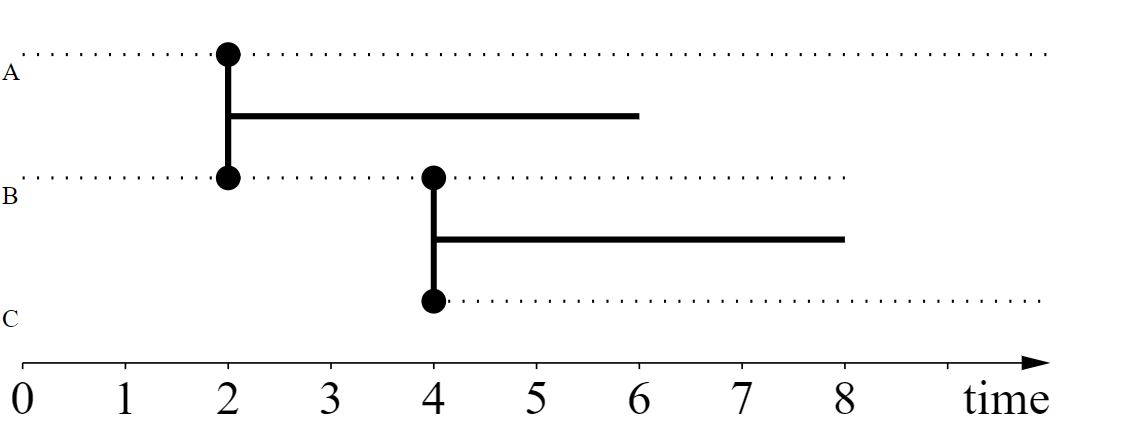
\includegraphics[width=0.5\textwidth]{exStreamGraph.JPG}
\caption{\textbf{Exemple de stream graph.} Dans cet exemple, on représente les interactions entre chercheurs durant une conférence de 10 heures ($T=[0,10]$). Les nœuds sont les trois chercheurs ($V=($MAP,MB,YYA$)$) et leurs intervalles d'existence sont les suivants $T_{\text{MAP}}=[4,10], T_{\text{MB}}=[0,10], T_{\text{YYA}}=[0,8]$, ils représente les moments où les chercheurs étaient présents à la conférence. Enfin les liens $V=([2,6]\times (\text{MB},\text{YYA})) \cup ([4,8]\times(\text{YYA},\text{MAP}))$ représentent les moments où les chercheurs ont discuté entre eux.}
\end{figure}




\subsubsection{Quelques définitions}

Dans l'article de référence \cite{stream}, de nombreuses notions sont ensuite définies de telle sorte à ce que dans le cas où le stream graph serait statique, on retrouve les mêmes notions que pour un graphe classique.

\paragraph{Mesures sur les stream graphes}

Dans \cite{stream}, on appelle \textbf{nombre de noeuds} $N_n(S)$ le nombre moyen de nœuds au cours du temps $N_n(S) = \sum_{u\in V}\frac{|T_u|}{|T|}$ et de la même façon le \textbf{nombre de liens} $N_e(S) = \sum_{e \in E} = \frac{|T_{u,v}|}{|T|}$.

La \textbf{densité} $d(S)$ est définie comme étant le nombre de noeuds sur le "nombre de noeuds possibles", c'est à dire :
$$
d(S) = \frac{\sum_{(u,v)\in E} |T_{u,v}|}{\sum_{(u,v)\in V\otimes V} |T_u \cap T_v|}
$$

L'\textbf{uniformité} est définie comme la probabilité que deux noeuds apparaissent en même temps dans le stream graph :

$$
 \Cup(S)=\sum_{u,v \in V \otimes V}\frac{|T_u\cap T_v|}{|T_u\cup T_v|}
$$

Un \textbf{cluster}

\paragraph{Chemins}


\section{Présentation d'un nouvel objet: le stream graph multicouche}



\subsection{Motivations}
\subsection{Définition}

\begin{defn}[\textbf{Stream graph multicouche}]
    
    Soit $T$ un intervalle de temps, ${\cal L}$ une structure de couches définie comme dans le cadre des graphes multicouches simples, et $V$ un ensemble de noeuds. 
    
    $T_M$ est un ensemble d'intervalles inclus dans $T$, indexé par les couches de $L$ et représente le temps d'existence de ces couches, avec pour contrainte que $\cup_{\alpha \in L} T_{\alpha} = T$ . $W_M$ est inclus dans $T \times V \times L$, et contient les temps d'existence de chaque nœud couche, sachant que le temps d'existence d'un nœud couche est forcément inclus dans le temps d'existence de la couche. Enfin, $E_M \subseteq T \times V \times L \times V \times L$ donne les liens entre les nœuds couches et leurs temps d'existence, sachant qu'un lien ne peut exister que pendant l'intersection des temps d'existence des nœuds-couches qu'il relie.
    
    L'objet $S_M = (T,T_M,V,W_M,E_M,{\cal L})$ est alors appelé \textbf{stream graph multicouches } (ou multilayer stream graph en anglais).
    
    On définit également les temps d'existence des noeuds-couches $T_{u,\alpha}$ et les temps d'existence des liens $T_{(u,\alpha),(v,\beta)}$ qui sont des unions d'intervalles.
	\end{defn}
	
	\begin{figure}[H]
		\centering
		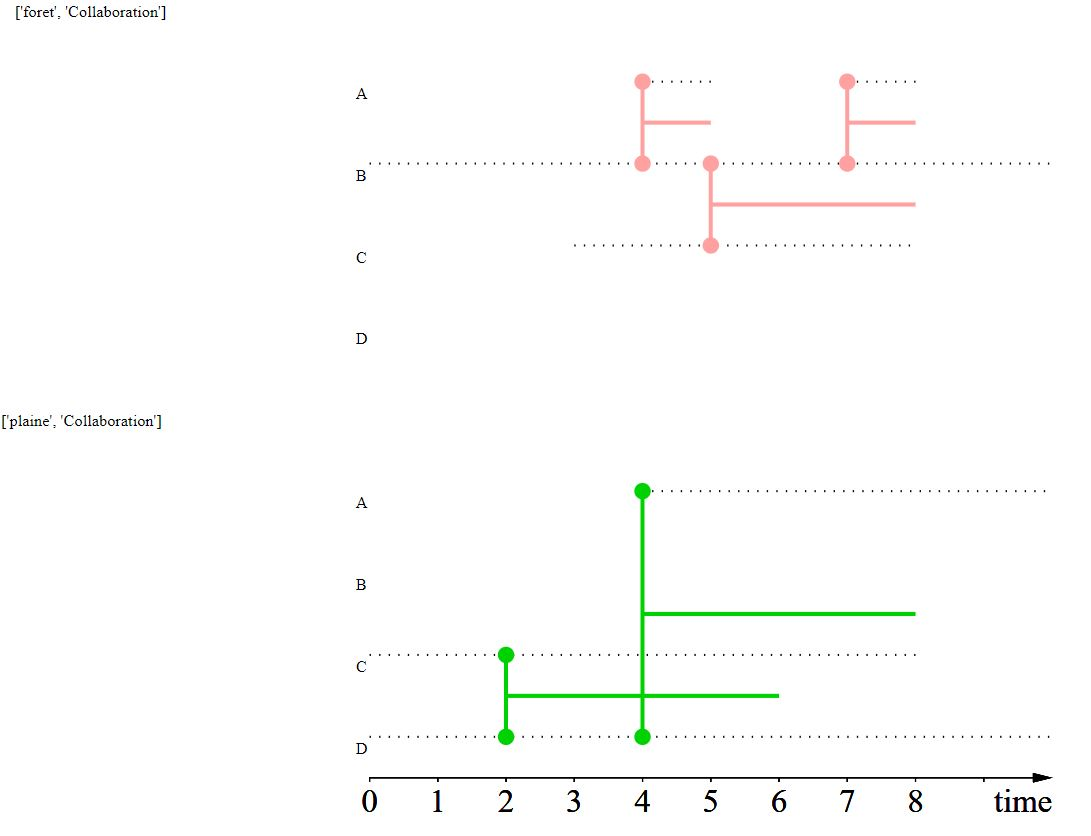
\includegraphics[width=0.8\textwidth]{exMultiStream.JPG}
		\caption{La représentation en multilayer stream graph des couches ["ECCS13","Talk to each other"] et ["Workshop in Oxford","Talk to each other"], générée avec "multiplex-stream" (description du programme en partie \ref{descode})}
	\end{figure}
	
	\begin{rmq}
		On peut s'interroger sur le bien-fondé d'utiliser l'objet stream graph pour rajouter l'aspect temporel aux graphes multicouches. En effet, dans \cite{mlkiv}, les auteurs évoquent l'idée d'un aspect "continu", pouvant représenter le temps. Mais cette idée ne semble pas avoir été beaucoup exploitée, car les outils développés pour manipuler les graphes multicouches sont principalement matriciels et donc faits pour traiter un nombre de couches fini. De plus, des outils ont été spécifiquement créés pour traiter les stream graphs et l'idée ici est de les exploiter.
	
	\end{rmq}

\subsection{Extraction de sous-graphes}






\subsection{Mesures}



\section{Application à des données concrètes}

\subsection{Structure de données et organisation du code} 
\label{descode}

	La gestion des flots de liens multicouche implique assez rapidement de gérer un grand nombre d'informations "imbriquées" : chaque couche contient des noeuds, qui apparaissent à des temps précis, ces noeud-couches sont reliés par des liens, eux-mêmes apparaissant à des temps précis...
	
	J'ai choisi de construire des classes python pour simplifier la gestion de telles données, et pour permettre de vérifier que le stream graph multicouche reste cohérent quand on le modifie.
	
	\begin{figure}[H]
		\centering
		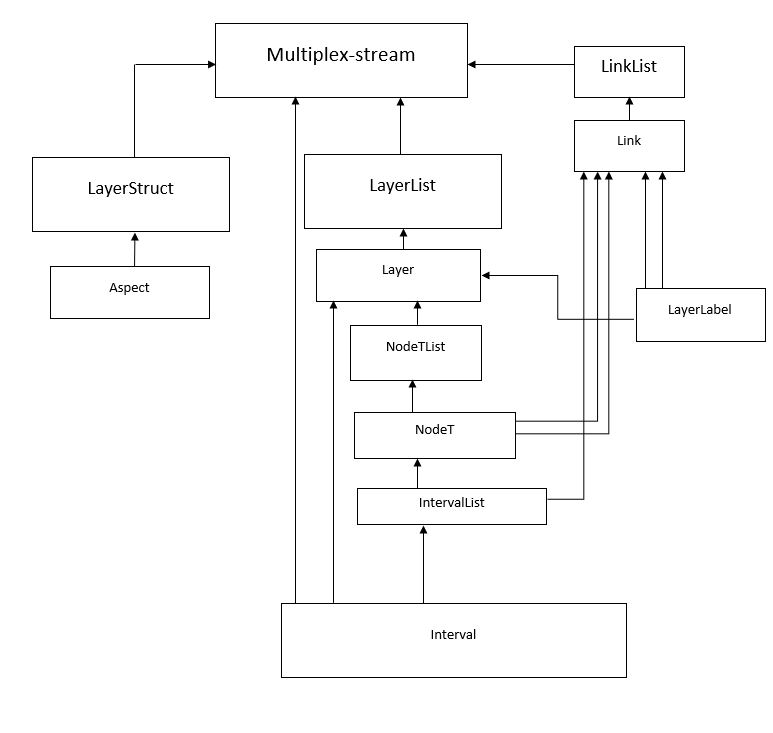
\includegraphics[width=0.5\textwidth]{codeStructure.JPG}
		\caption{Structure des classes de la }
	\end{figure}

\subsection{Classes préparatoires}
\subsection{Star Wars}
\subsection{Avions ?}

\section{Conclusions et perspectives}

    \nocite{*}
    \bibliographystyle{plain}
	\bibliography{rapport}

\end{document}
